\section{Auswertung}
\label{sec:Auswertung}

Für die Auswertung wurde Python und im Speziellen Matplotlib \cite{matplotlib}, SciPy \cite{scipy},
Uncertainties \cite{uncertainties} und NumPy \cite{numpy} verwendet.

\subsection{Einstellung des Selektivverstärkers}
In Tabelle \ref{taba} sind die Frequenzen $\nu$ und die jeweils gemessenen Ausgangspannungen $U_\text{A}$ 
bei einer Eingangsspannung von $U_\text{E} = \SI{100}{\milli\volt}$ eingetragen. 
In Abb. \ref{plota} sind diese Werte gegeneinander aufgetragen.

\begin{table}\caption{Die Länge der Zylinder und die Spannung mit den jeweiligen Zeitenpunkten der Ausschläge.}
\label{taba}
\centering
\sisetup{round-mode = places, round-precision=2, round-integer-to-decimal=true}
\begin{tabular}{S[]S[]S[]S[]S[]} 
\toprule
{$l/ \si{\milli\meter}$} & {$U_1/ \si{\volt}$} & {$t_1/ \si{\micro\second}$} & {$U_2/ \si{\volt}$} & {$t_2/ \si{\micro\second}$}\\
\midrule
120.8 & 1.29 & 0.6 & 0.17 & 88.7\\
102.3 & 1.27 & 0.5 & 0.2 & 76.5\\
80.5 & 1.33 & 0.6 & 0.76 & 59.8\\
40.4 & 1.33 & 0.5 & 1.34 & 30.2\\
31.1 & 1.29 & 0.5 & 1.37 & 23.8\\
\bottomrule
\end{tabular}\end{table}

% Plot einfügen 
\begin{figure}
    \centering
    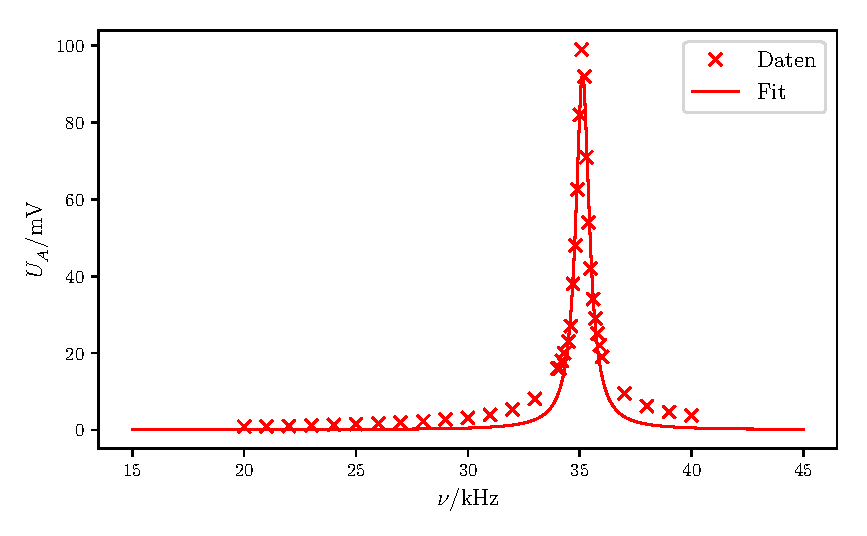
\includegraphics[width=15cm, height=8cm]{build/plota2.pdf} %
    \caption{Die Filterkurve des Selektivverstärkers. Die Ausgangspannung $U_\text{A}$
    ist gegen die Frequenz $\nu$ aufgetragen. Es sind die Daten und ein Fit eingetragen.}
    \label{plota}
\end{figure}

\noindent Der Fit wurde mit Gleichung \eqref{cauchyverteilung} gefittet. Die Werte, die sich daraus ergeben, sind
\begin{align*} 
  a &= \SI{106.38(289)}{\milli\volt\kilo\hertz} \\
  s &= \SI{0.37(2)}{\kilo\hertz} \\
  t &= \SI{35.13(1)}{\kilo\hertz}. 
\end{align*}


\noindent Aus der Tabelle lassen sich der Wert $\nu_0$ und die beiden Werte $\nu_\text{-}$ und $\nu_\text{+}$ ungefähr ablesen.
Da das Maximum bei $\SI{99}{\milli\volt}$ liegt, liegen die anderen beiden Frequenzen auf der Höhe von $\SI{70.004}{\milli\volt}$.
Die Werte ergeben sich zu 
\begin{align*} 
 \nu_0 &= \SI{35.1}{\kilo\hertz} \\
 \nu_{-} &= \SI{34.95}{\kilo\hertz} \\
 \nu_{+} &= \SI{35.3}{\kilo\hertz}. 
\end{align*}

\noindent Daraus lässt sich mit Gleichung \eqref{eqn:guete} erkennen, dass die Güte den Wert 
\begin{align*} 
    Q_\text{exp} = \num{100.286}
\end{align*}
hat. 

\noindent Der gegebene Wert für $Q$ liegt bei 
\begin{align*} 
    Q = \num{100}.
\end{align*}


\subsection{Theoretische Suszeptibilität} 
Für die verschiedenen Stoffe haben sich aufgrund der verschiedenen Elemente und Zusammensetzungen auch verschiedene 
Werte für die Suszeptibilität ergeben. 
Die Werte, die zur Berechnung nötig waren, sind die Temperatur $T$, die als Raumtemperatur von $\SI{20}{\celsius}$ angenommen wurde, was einem Wert von \SI{293.15}{\kelvin} entspricht. 

\noindent Die Anzahl der Momente N wurde mit der Formel \eqref{N} berechnet. Dafür wurde die Dichte $\rho$ und die Molmasse $M$ benötigt. Um $Q_{real}$ zu bestimmen, wird auch noch die tatsächliche Masse der jeweiligen Stoffe benötigt. Alle drei Werte sind in Tab. \ref{tab2} eingetragen.
Die Dichten und Massen der unteren drei Elemente sind der Anleitung \cite{V606} sowie der Beschriftung auf den Proben entnommen.
Die Molmasse des ersten Elements stammt von einem Rechner für Molare Masse \cite{C6}.

\begin{table}\caption{Das Verhältnis des magnetischen Feldes durch die Beschleunigungsspannung aufgetragen gegen die Höhe.}
\label{tab2}
\centering
\sisetup{round-mode = places, round-precision=2, round-integer-to-decimal=true}
\begin{tabular}{S[]S[]S[]} 
\toprule
{$B_1 / \si{\henry}$} & {$B_2 / \si{\henry}$} & {$\frac{D}{(L^2 + D^2)} / \si{\per\meter}$}\\
\midrule
0.0 & 0.0 & 0.0\\
3.5649278338607584e-07 & 3.862005153349155e-07 & 0.29289724188430566\\
8.912319584651897e-07 & 8.912319584651897e-07 & 0.5827222842713544\\
1.4259711335443034e-06 & 1.396263401595464e-06 & 0.8665094112549946\\
1.9250610302848096e-06 & 1.8418793808280586e-06 & 1.1414982164090373\\
2.3885016486867084e-06 & 2.3172030920094934e-06 & 1.4052180429996723\\
2.923240823765822e-06 & 2.822234535139767e-06 & 1.6555530006898145\\
3.4223307205063282e-06 & 3.3272659782700412e-06 & 1.8907846756403912\\
\bottomrule
\end{tabular}\end{table}

\noindent Für den Stoff $Nd_2 O_3$ ergibt sich die konkrete Rechnung des Landé-Faktors $g_J$ folgendermaßen: 

\begin{align*}
    g_J &= \frac{3 J (J+1) + S (S+1) - L (L+1)}{2 J (J+1)} \\
        &= \frac{3 \cdot 4,5 \cdot(4,5 + 1) + 1,5 \cdot (1,5 +1) - 6 \cdot (6+1)}{2 \cdot 4,5 \cdot (4,5 + 1)} \\
        &= 0,73.
\end{align*} 

\noindent Der Wert für $S$ ergibt sich, da wir \num{3} Elektronen auf der $4f$ Schale haben, die sich nach der ersten Hundschen Regel erstmal alle parallel ausrichten und sich somit zu einem Spin von $S = \frac{1}{2}+ \frac{1}{2} + \frac{1}{2}$ ergeben. Nach der zweiten Regel dürfen sie nicht den gleichen Drehimpuls $l$ besitzen. So ergibt sich, dass $L = 3 + 2 + 1$ ist. 

\noindent Die anderen drei Werte lassen sich analog ermitteln. 
In Tab. \ref{tab1} befinden sich die Werte für $L$, $S$ und $J$. Daneben stehen jeweils die Werte, die sich für 
$g_J$ ergeben. 

\begin{table}\caption{Der maximale Drehimpuls $L$, der Gesamtspin $S$ und der Gesamtdrehimpuls $J$ ergeben sich zum Landé-Faktor $g_\text{J}$ für die vier verschiedenen Elemente.}
\label{tab1}
\centering
\sisetup{round-mode = places, round-precision=2, round-integer-to-decimal=true}
\begin{tabular}{S[]S[]S[]S[]} 
\toprule
{$L$} & {$S$} & {$J$} & {$g_\text{J}$}\\
\midrule
5.0 & 1.0 & 4.0 & 0.8\\
0.0 & 3.5 & 3.5 & 2.0\\
6.0 & 1.5 & 4.5 & 0.7272727272727273\\
5.0 & 2.5 & 7.5 & 1.3333333333333333\\
\bottomrule
\end{tabular}\end{table} %falsche Tabelle

\noindent Die Werte für die Suszeptibilität, die mittels Gleichung \eqref{eqn:chitheo} berechnet werden können, ergeben sich für die jeweiligen Stoffe 
zu folgenden Werten 

\begin{align*} 
   \chi_{C_6 O_{12} Pr_2} &= \num{24.6e-5}\\
   \chi_{Gd_2 O_3} &= \num{1158.9e-5}\\
   \chi_{Nd_2 O_3} &= \num{280.3e-5}\\
   \chi_{Dy_2 O_3} &= \num{2816.6e-5}.
\end{align*}

\subsection{Suszeptibilität mittels Spannungsverhältnis}
In Tab. \ref{tab3} sind die Spannungsdifferenzen vor und nach dem Einlegen der Probe und daneben die Widerstandsdifferenzen beim gleichen Vorgang für die verschiedenen Elemente aufgelistet.

\begin{table}\caption{Der Winkel \varphi gegen die Stromstärke I aufgetragen.}
\label{tab1}
\centering
\sisetup{round-mode = places, round-precision=2, round-integer-to-decimal=true}
\begin{tabular}{S[]S[]} 
\toprule
{$\varphi / \si{\milli\radian}$} & {$I / \si{\nano\ampere}$}\\
\midrule
-12.577953012282642 & 1.0999999999999999\\
-12.353369766296458 & 0.8999999999999998\\
-12.128785274090491 & 1.1999999999999995\\
-11.904199558309829 & 1.7\\
-11.679612641600295 & 1.8\\
-11.455024546608442 & 1.1999999999999995\\
-11.230435295981538 & 1.1999999999999995\\
-11.005844912367545 & 1.8\\
-10.781253418415117 & 2.499999999999999\\
-10.556660836773576 & 1.9000000000000001\\
-10.332067190092905 & 1.1999999999999995\\
-10.107472501023729 & 1.6000000000000003\\
-9.882876792217305 & 2.9000000000000004\\
-9.658280086325508 & 3.1000000000000005\\
-9.433682406000813 & 1.8\\
-9.20908377389629 & 1.1999999999999995\\
-8.984484212665583 & 2.3\\
-8.759883744962893 & 3.6\\
-8.53528239344298 & 2.9000000000000004\\
-8.310680180761132 & 1.6000000000000003\\
-8.086077129573162 & 1.6000000000000003\\
-7.861473262535383 & 2.9000000000000004\\
-7.636868602304612 & 3.1000000000000005\\
-7.41226317153814 & 2.0\\
-7.187656992893724 & 1.4000000000000001\\
-6.963050089029578 & 2.1\\
-6.738442482604351 & 2.6\\
-6.513834196277122 & 1.9000000000000001\\
-6.289225252707374 & 1.2999999999999996\\
-6.064615674554994 & 1.6000000000000003\\
-5.840005484480253 & 2.4\\
-5.61539470514379 & 2.3\\
-5.3907833592066 & 1.6000000000000003\\
-5.166171469330024 & 1.6000000000000003\\
-4.941559058175732 & 2.4\\
-4.716946148405708 & 3.3000000000000007\\
-4.492332762682237 & 3.7\\
-4.2677189236678945 & 3.1999999999999997\\
-4.043104654025528 & 3.1000000000000005\\
-3.8184899764182507 & 4.199999999999999\\
-3.5938749135094157 & 6.1000000000000005\\
-3.369259487962614 & 7.599999999999999\\
-3.1446437224416557 & 6.599999999999999\\
-2.920027639610556 & 5.6000000000000005\\
-2.6954112621335216 & 7.000000000000001\\
-2.4707946126749376 & 10.4\\
-2.2461777138993564 & 12.400000000000002\\
-2.0215605884714787 & 10.4\\
-1.7969432590561418 & 8.399999999999999\\
-1.572325748318309 & 10.4\\
-1.3477080789230522 & 15.399999999999999\\
-1.123090273535539 & 16.400000000000002\\
-0.8984723548210195 & 13.4\\
-0.673854345444813 & 10.4\\
-0.44923626807229305 & 13.4\\
-0.22461814536887456 & 17.4\\
0.22461814536887456 & 13.4\\
0.44923626807229305 & 11.4\\
0.673854345444813 & 14.4\\
0.8984723548210195 & 17.4\\
1.123090273535539 & 15.399999999999999\\
1.3477080789230522 & 11.4\\
1.572325748318309 & 10.4\\
1.7969432590561418 & 12.400000000000002\\
2.0215605884714787 & 14.4\\
2.2461777138993564 & 11.4\\
2.4707946126749376 & 8.399999999999999\\
2.6954112621335216 & 8.399999999999999\\
2.920027639610556 & 10.4\\
3.1446437224416557 & 9.400000000000002\\
3.369259487962614 & 6.800000000000001\\
3.5938749135094157 & 5.5\\
3.8184899764182507 & 7.400000000000001\\
4.043104654025528 & 8.200000000000001\\
4.2677189236678945 & 6.2\\
4.492332762682237 & 4.199999999999999\\
4.716946148405708 & 4.9\\
4.941559058175732 & 6.599999999999999\\
5.166171469330024 & 6.1000000000000005\\
5.3907833592066 & 4.300000000000001\\
5.61539470514379 & 4.1000000000000005\\
5.840005484480253 & 5.6000000000000005\\
6.064615674554994 & 6.0\\
6.289225252707374 & 4.7\\
6.513834196277122 & 4.1000000000000005\\
6.738442482604351 & 5.2\\
6.963050089029578 & 5.9\\
7.187656992893724 & 4.9\\
7.41226317153814 & 3.8000000000000003\\
7.636868602304612 & 4.4\\
7.861473262535383 & 5.4\\
8.086077129573162 & 4.9\\
8.310680180761132 & 3.3000000000000007\\
8.53528239344298 & 2.9999999999999996\\
8.759883744962893 & 3.8000000000000003\\
8.984484212665583 & 3.9999999999999996\\
9.20908377389629 & 2.9999999999999996\\
9.433682406000813 & 2.0\\
9.658280086325508 & 2.0\\
9.882876792217305 & 2.3\\
10.107472501023729 & 2.0\\
10.332067190092905 & 1.5000000000000002\\
10.556660836773576 & 1.2999999999999996\\
10.781253418415117 & 1.0999999999999999\\
11.005844912367545 & 0.9999999999999999\\
11.230435295981538 & 0.8999999999999998\\
11.455024546608442 & 0.9999999999999999\\
11.679612641600295 & 0.9999999999999999\\
11.904199558309829 & 0.8999999999999998\\
12.128785274090491 & 0.6999999999999996\\
12.353369766296458 & 0.6999999999999996\\
12.577953012282642 & 0.8999999999999998\\
12.802534989404709 & 1.0999999999999999\\
13.027115675019099 & 1.0999999999999999\\
13.251695046483025 & 0.8999999999999998\\
13.476273081154504 & 0.6999999999999996\\
13.70084975639236 & 0.9999999999999999\\
13.925425049556234 & 1.2999999999999996\\
14.14999893800661 & 1.2999999999999996\\
14.374571399104815 & 0.9999999999999999\\
\bottomrule
\end{tabular}\end{table}
\noindent Die Werte für die Suszeptibilität, die mittels Gleichung \eqref{eqn:chiexp1} berechnet werden können, ergeben sich für die jeweiligen Stoffe 
zu folgenden Werten 

\begin{align*} 
   \chi_{C_6 O_{12} Pr_2} &= \num{1.2(6)e-5}\\
   \chi_{Gd_2 O_3} &= \num{268.0(17)e-5}\\
   \chi_{Nd_2 O_3} &= \num{15(4)e-5}\\
   \chi_{Dy_2 O_3} &= \num{703(9)e-5}.
\end{align*}


\subsection{Suszeptibilität mittels Widerstandsverhältnis}
Mit Gleichung \eqref{eqn:chiexp2} und den Werten aus Tab. \ref{tab3}
wird die Suszeptibilität der Proben bestimmt.
Es ergeben sich die Werte

\begin{align*} 
   \chi_{C_6 O_{12} Pr_2} &= \num{18(8)e-5}\\
   \chi_{Gd_2 O_3} &= \num{980(17)e-5}\\
   \chi_{Nd_2 O_3} &= \num{190(18)e-5}\\
   \chi_{Dy_2 O_3} &= \num{2302(20)e-2}.
\end{align*}